\documentclass[10 pt]{article}

\usepackage[utf8x]{inputenc}
\usepackage{dsfont}
\usepackage{amsthm}
\usepackage{amsfonts}
\usepackage{amssymb}
\usepackage{tensor}
\usepackage{mathtools}
\usepackage[T1]{fontenc}
%\usepackage[spanish]{babel}
\usepackage[cm]{fullpage}
\usepackage{graphicx}
\usepackage{float}
\usepackage{bm}
\usepackage{setspace}
\usepackage{enumitem}
\usepackage{mdwlist}
\usepackage{parskip}
\usepackage{listings}
\usepackage{color}
%\usepackage{epstopdf}
\usepackage{tikz,datatool}
\usepackage{hyperref}

\newcommand{\HRule}{\rule{\linewidth}{0.5mm}}

\AtBeginDocument{
  \let\myThePage\thepage
  \renewcommand{\thepage}{\oldstylenums{\myThePage}}
}

\newcommand{\gra}{$^\text{o}$}
\newcommand{\dif}{\text{d}}
\newcommand{\avg}[1]{\left\langle #1 \right\rangle}
\newcommand{\ket}[1]{\left| #1 \right\rangle}
\newcommand{\bra}[1]{\left\langle #1 \right|}
\newcommand{\bket}[2]{\left\langle #1 \middle| #2 \right\rangle}
\newcommand{\der}[2]{\frac{\text{d} #1}{\text{d} #2}}
\newcommand{\prt}[2]{\frac{\partial #1}{\partial #2}}
\newcommand{\dert}[3]{\frac{\text{d}^#3 #1}{\text{d} #2^#3}}
\newcommand{\prtt}[3]{\frac{\partial^#3 #1}{\partial #2^#3}}
\newcommand{\dl}{\mathcal{L}}
\newcommand{\dha}{\mathcal{H}}
\newcommand{\vol}{\text{vol}}
\renewcommand{\vec}[1]{\pmb{#1}}

\newenvironment{algo}[1]
{  \begin{center}
   \mbox{
       \begin{minipage}{\textwidth}
           \begin{tabbing}
           \settabs
            #1
           \end{tabbing}
        \end{minipage}
    }
    \end{center}
}{}
\newcommand{\settabs}{mmm\=mmm\=mmm\=mmm\=mmm\=mmm\=\kill}

\DeclarePairedDelimiter\ceil{\lceil}{\rceil}
\DeclarePairedDelimiter\floor{\lfloor}{\rfloor}

\definecolor{mygray}{rgb}{0.4,0.4,0.4}
\definecolor{mygreen}{rgb}{0,0.5,0.25}
\definecolor{myorange}{rgb}{1.0,0.4,0}

\definecolor{clock0}{cmyk}{1,0,0,0}
\definecolor{clock1}{cmyk}{1,1,0,0}
\definecolor{clock2}{cmyk}{0,1,0,0}
\definecolor{clock3}{cmyk}{0,1,1,0}
\definecolor{clock4}{cmyk}{1,0,1,0}
\definecolor{clock5}{cmyk}{1,1,1,0}
\definecolor{clock6}{cmyk}{0,0,1,0}
\definecolor{clock7}{cmyk}{0,0,0,0.1}

\begin{document}

\lstset{
language=C++,
basicstyle=\ttfamily\color{black},
commentstyle=\color{mygray}\ttfamily,
frame=single,
numbers=left,
numbersep=5pt,
numberstyle=\tiny\color{mygray}\ttfamily,
keywordstyle=\color{mygreen}\ttfamily,
showspaces=false,
showstringspaces=false,
stringstyle=\color{myorange}\ttfamily,
tabsize=2,
emph={double,uint8_t,uint16_t,uint32_t,uint64_t,int8_t,int16_t,int32_t,int64_t},
emphstyle={\color{blue}\ttfamily}
}

\begin{center}
  \Large \textsc{Week 6: MC simulation of a Lennard-Jones fluid in the NVT ensemble}
\end{center}

\begin{center}
  \large \textsc{Francisco García Flórez}
\end{center}

\section{Pressure}

\subsection{Pressure with the first Virial term}

From the Virial theorem we know the pressure of the system can be written as

$$ \avg{P} = \rho k_B T + \avg{\sum_{i<j} \vec{f}(\vec{r}_{ij}) \cdot \vec{r}_{ij}} \text{ ,} $$

where $\vec{r}_{ij}$ is the vector distance between two particles of the system, considering the boundary conditions. The force $\vec{f}(\vec{r})$ will in this case be computed from a potential, specifically the \emph{truncated and shifted} Lennard-Jones potential, given by:

$$ u(r_{ij}) = \left\{
    \begin{alignedat}{2}
      4 \epsilon \left[ \left( \frac{\sigma}{r_{ij}} \right)^{12} - \left( \frac{\sigma}{r_{ij}} \right)^6 \right] - \epsilon_{\text{cut}} ~~, & ~~ r_{ij} \leq r_{\text{cut}} \\
      0 ~~, & ~~ r_{ij} > r_{\text{cut}} \\
    \end{alignedat}
  \right. ~~, ~~ \epsilon_{\text{cut}} =  4 \epsilon \left[ \left( \frac{\sigma}{r_{\text{cut}}} \right)^{12} - \left( \frac{\sigma}{r_{\text{cut}}} \right)^6 \right] \text{ .}
$$

Where in this case $r_{ij}$ is the scalar distance between two particles. As usual, the force exerted by this potential can be computed by $\vec{f}(\vec{r}_{ij}) = \vec{\nabla} u(r_{ij})$, which in this case reduces to

$$ \vec{f}(\vec{r}_{ij}) = \vec{\nabla} u(r_{ij}) = \frac{1}{r_{ij}} \der{u(r_{ij})}{r_{ij}} \vec{r}_{ij} \text{ .} $$

Thus, plugging it in $\avg{P}$:

$$ \avg{P} =
  \rho k_B T + \avg{\sum_{i<j} \frac{1}{r_{ij}} \der{u(r_{ij})}{r_{ij}} \vec{r}_{ij} \cdot \vec{r}_{ij}} =
  \rho k_B T + \avg{\sum_{i<j} \der{u(r_{ij})}{r_{ij}} r_{ij}} =
  \rho k_B T + \avg{\sum_{i<j} 24 \epsilon \left[ 2 \left( \frac{\sigma}{r_{ij}} \right)^{12} - \left( \frac{\sigma}{r_{ij}} \right)^6 \right]} \text{ ,}
$$

where we have assumed $r_{ij} \leq r_\text{cut}$ for simplicity, as it would be zero otherwise. It's straightforward to see now that the function in the program computes precisely this second term. Notice that this procedure is not valid for other potentials like Hard Spheres, since in that case the Virial term will be always zero, so the pressure we would compute is the same as that of the ideal gas, which clearly does not describe a system of Hard Spheres in general.

\subsection{Results}

In the following plots we show the results for the Pressure as a function of Density.

\begin{figure}[H]
  \begin{center}
    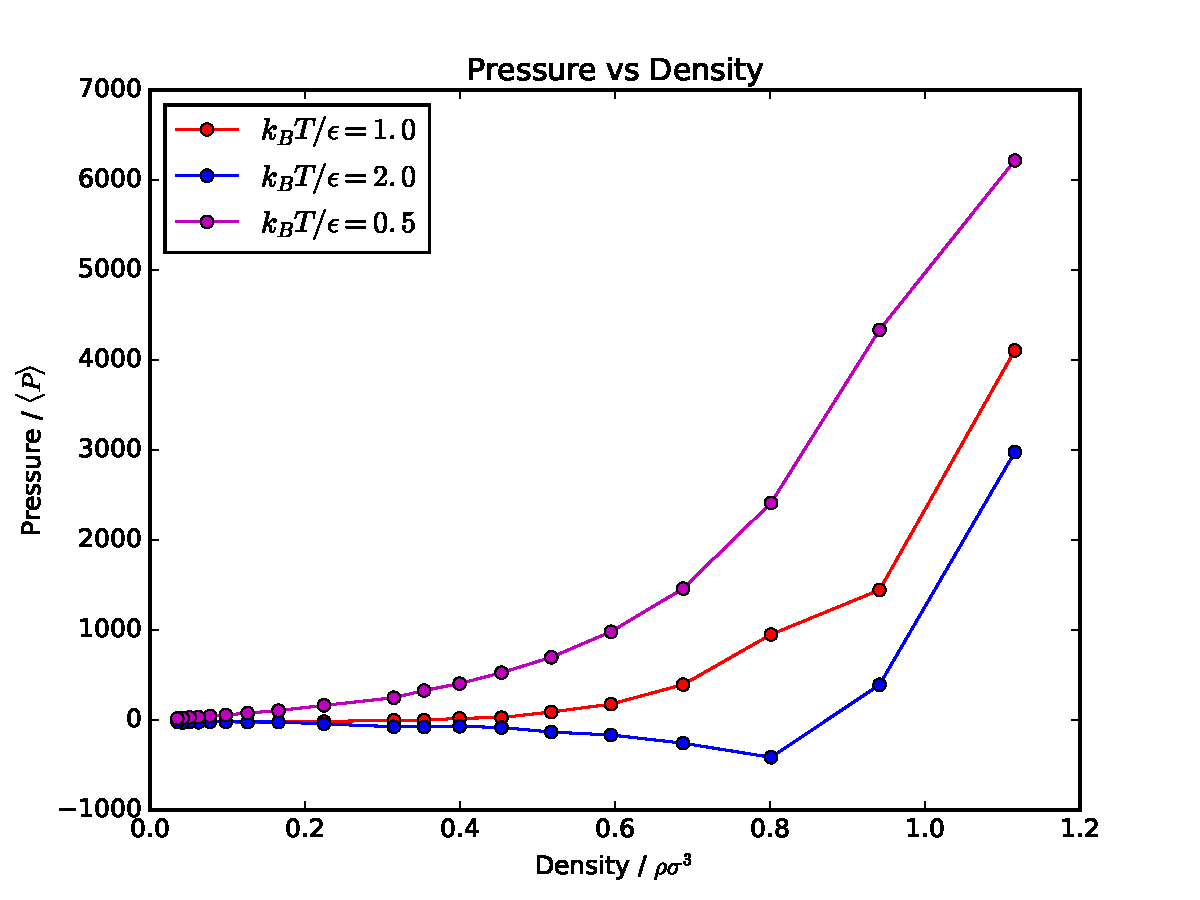
\includegraphics[width=0.49\textwidth]{{../graphs/P_rho}.pdf}
    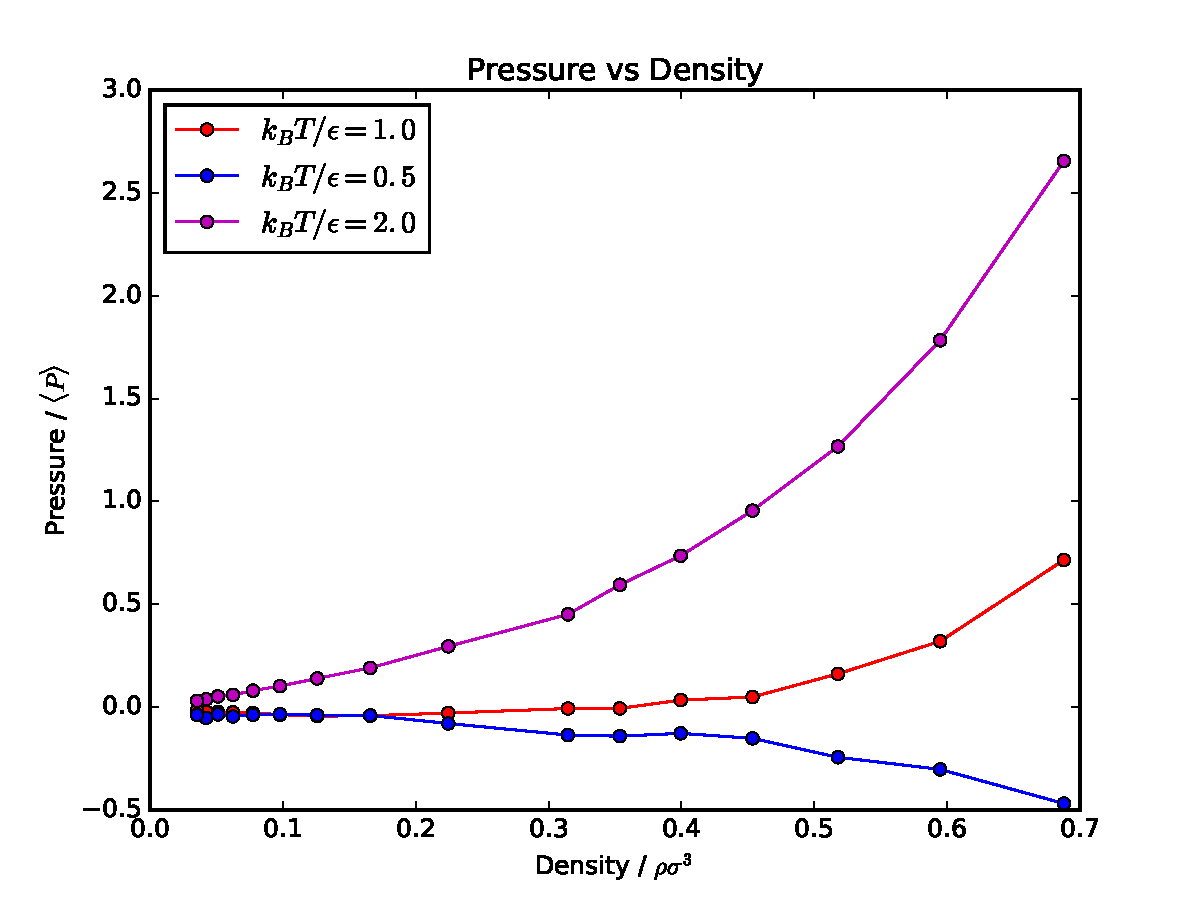
\includegraphics[width=0.49\textwidth]{{../graphs/P_rho_b}.pdf}
  \end{center}
  \caption{Plot of the pressure as a function of density, (left) full range and (right) closer look.}
\end{figure}

As we could have expected, for high densities the pressure increases significantly and becomes clearly non-linear, since we would be dealing with a solid phase. On the other hand, looking at the right plot for low densities its behavior is more linear, as we would expect from an ideal gas of weakly interacting particles. Although, this approximation is only valid for $\rho \sigma^3 \lesssim 0.25$.

On the other hand, for high values of $T^*$ and density $\rho \sigma^3 \sim 0.8$ we can see a slight valley and a change in the sign of the derivative. This behavior could mean a phase change from fluid to solid, but more analysis would be required to get more information.

\section{Chemical Potential $\mu$}

\subsection{Chemical Potential and Hard Spheres}

In this program we are computing the excess chemical potential $\mu_{ex}$ by testing the insertion of a particle in the system, called the Widom test. In this way $\mu_{ex}$ can be computed using

$$ \mu_{ex} = - k_B T \log\left( \sum_{i=1}^{N_\text{test}} \frac{\exp[-\beta \Delta U_i^+]}{N_\text{test}} \right) \text{ .} $$

However, as before this method wouldn't give good results used with Hard Spheres, since the change in energy $\Delta U_i^+$ will always be zero or $\infty$, and therefore this formula will not give physically correct results.

\subsection{Results}

In the following plots we show the results for the $\mu_{ex}$ as a function of Density.

\begin{figure}[H]
  \begin{center}
    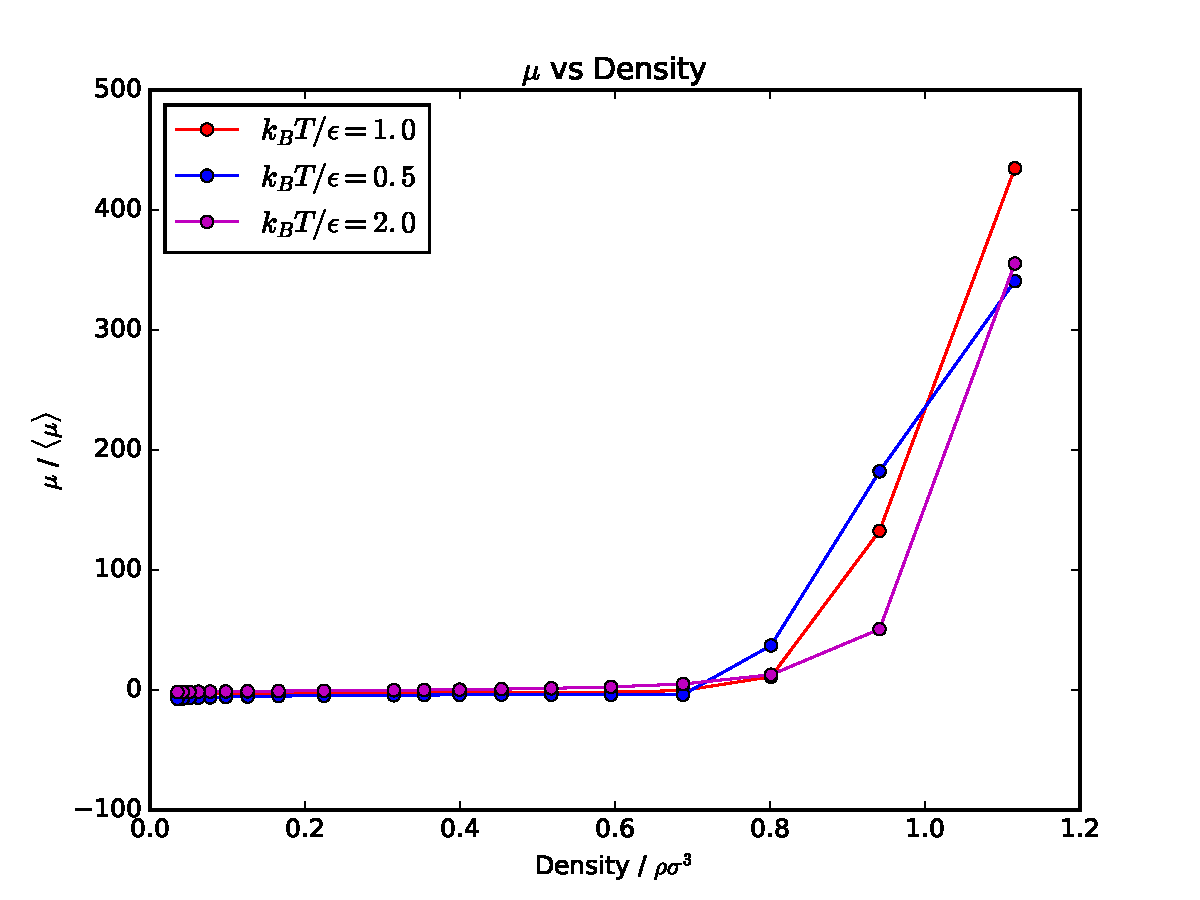
\includegraphics[width=0.49\textwidth]{{../graphs/mu_rho}.pdf}
    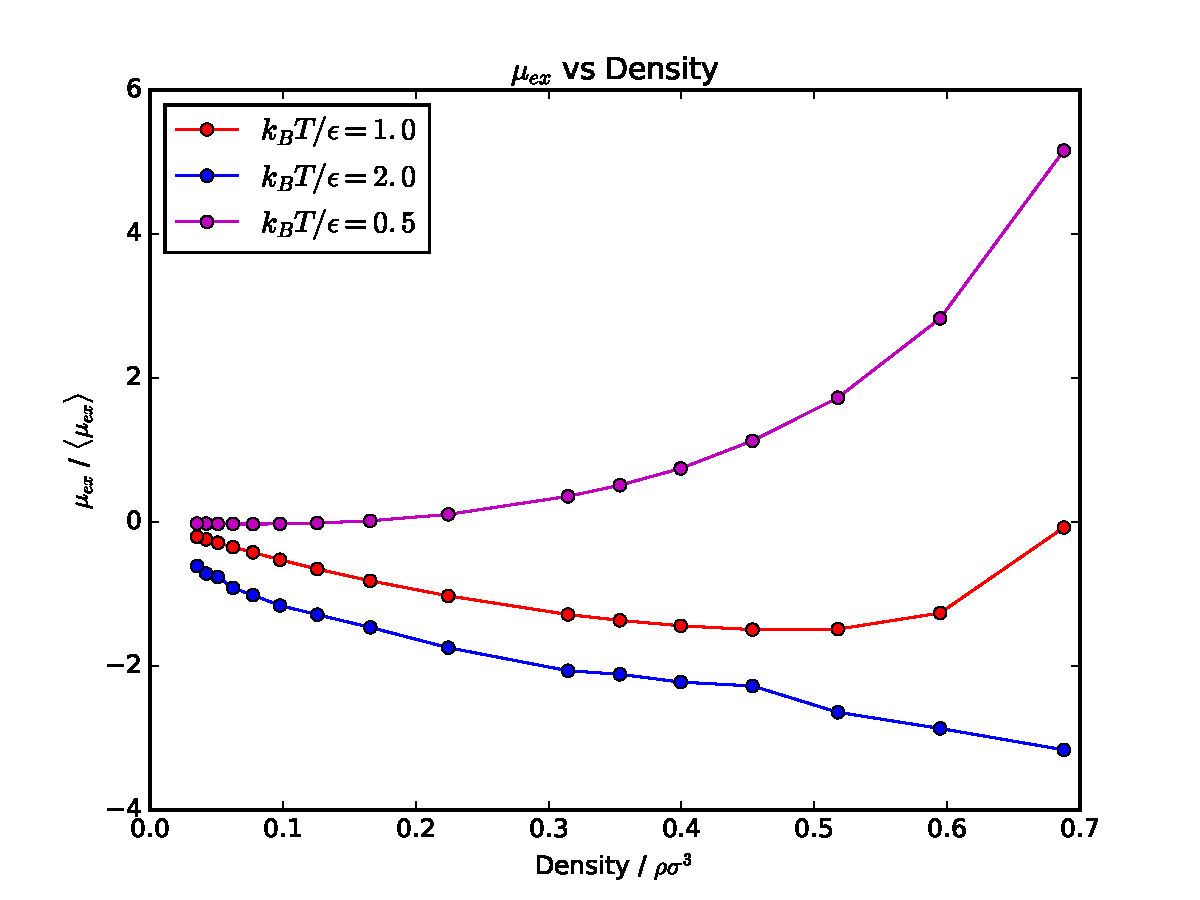
\includegraphics[width=0.49\textwidth]{{../graphs/mu_rho_b}.pdf}
  \end{center}
  \caption{Plot of the $\mu_{ex}$ as a function of density, (left) full range and (right) closer look.}
\end{figure}



\end{document}
